\chapter{Introduction}
\label{sec:introduction}
This chapter will introduce the subject of mixed criticality embedded systems and the project to the reader.

\section{Background}
Today, modern automotive systems contain a large number of Electronic Control Units (ECU)s \cite{}, each controlling a specific system of a specific criticality level such as safety-critical distance keeping system (\ref{sec:platooning}) or non-critical entertainment systems \cite{}. This approach provides isolation for the numerous critical and non-critical applications in the collective system, and a simple mechanism to qualify an individual ECU. However, it yields an inefficient use of system resources \cite{} and expensive system implementation \cite{}. In order to lower the cost of the system and increase system efficiency, applications of different criticality levels can be integrated into a single multicore platform, leading to a Mixed Criticality System (MCS). However, this approach increases system complexity, and hinders the certification of safety-critical systems \cite{}. In order to facilitate the design, test, and certification of such systems, spatial and temporal partitioning can be used in the architecture of the system as described by \cite{zaki2016}.\\

MCS

\subsection{Definition of safety-critical systems}
The term "Safety-critical system" has many definitions, most quite similar. Most definitions relate to systems with the potential to harm humans if the system malfunctions. According to \cite{website:encyclopedia} it is defined as "A system in which any failure or design error has the potential to lead to loss of life." Further, \cite{website:dictionary} defines safety-critical systems as "A computer, electronic or electromechanical system whose failure may cause injury or death to human beings." A Wikipedia article, \cite{website:wikipedia}, defines a safety-critical system (or "life-critical system") as a system whose failure or malfunction may result in one (or more) of the following outcomes:
\begin{itemize}
\item death or serious injury to people
\item loss or severe damage to equipment/property
\item environmental harm
\end{itemize}
In this thesis, a safety-critical system will be defined as "a system whose failure may cause injury or death to human beings."

\subsection{EMC2 Mixed criticality embedded system}
\label{sec:mces}
The current MCS is implemented on a Xilinx Zynq-7000. It employs two operating systems to handle applications of different criticality. A Linux General Purpose Operating System (GPOS) for non-safety critical applications and a Real-Time Operating System for safety-critical applications. Hypervisor, FPGA, peripherals

An overview of the system can be seen in Figure~\ref{fig:introduction_overview}.

\begin{figure}[H]
\centering
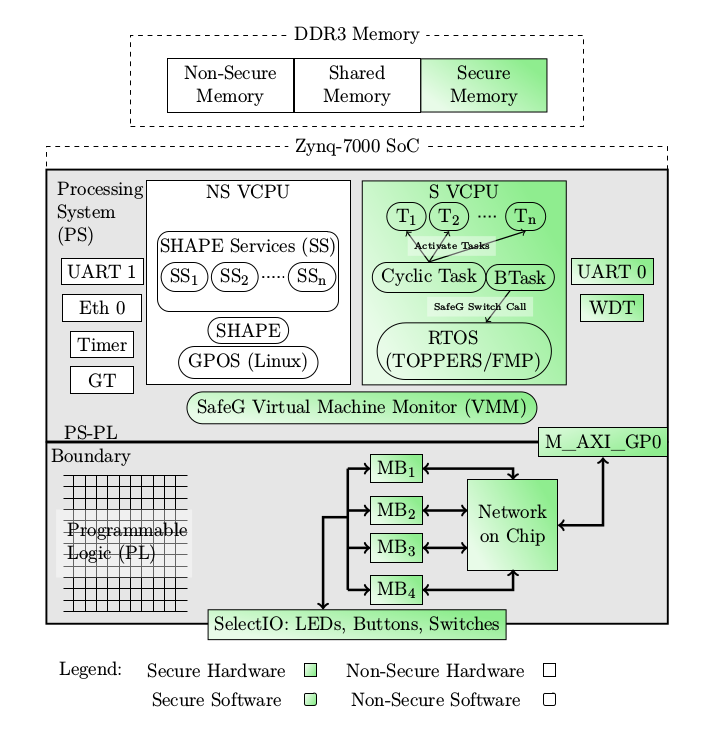
\includegraphics[width=\textwidth]{./img/introduction_overview.png}
\caption{System overview of the MCS in place.\cite{zaki2016}}\label{fig:introduction_overview}
\end{figure}

For more detailed information, see the entire report by \cite{zaki2016}.

\subsection{Platooning}
\label{sec:platooning}
Describe platooning.

\section{Problem statement}
\label{sec:problem}
%Implement safety-critical controller on the embedded system. 
A distance keeping control algorithm for platooning will be implemented on the embedded system described in \ref{sec:mces}. A demonstrator will be constructed in the form of a RC car capable of following a vehicle in front of it at a certain distance. It should be verified that no matter the computational load and eventual crashes of the Linux based non-critical system, the distance keeping algorithm on the RTOS never crashes. The performance of the control system should be measured and compared with the same controller without any non-critical computational load. Missed deadlines? CPU usage? Evaluate different scheduling methods.\\

This problem leads to the research question: 
\begin{itemize}
\item How well can a safety-critical control system perform when implemented on a mixed criticality system using virtualization?
\end{itemize}
alternatively:
\begin{itemize}
\item How, in a disciplined way, to reconcile the conflicting requirements of partitioning for safety assurance and sharing for efficient resource usage? \cite{burns2016}
\end{itemize}
alternatively:
\begin{itemize}
\item Is virtualization an efficient approach when trying to reconcile the conflicting requirements of partitioning for safety assurance and sharing for efficient resource usage when implementing a safety-critical control system?
\end{itemize}

\section{Purpose}
Protecting the integrity of a component from the faults of another is desired in all systems hosting multiple applications. However, it is of higher significance if the different applications have different criticality levels. Without such protection all components on the same system would need to be engineered to the standards of the highest criticality level, potentially massively increasing development costs \cite{burns2016}.

Reducing the amount of computers in automotive systems would have many effects. Manufacturing costs would decrease and with fewer physical components maintenance costs would also decrease. However, the system complexity would increase and thereby increasing time and cost to design the system. %Also,

%In order to reduce the amount of ECUs in mechatronic systems, it must be verified that non safety critical applications do not interfere with safety critical applications.

\section{Goals}
In this project there are both team goals and individual goals that do not necessarily align with each other. 

\subsection{Team goal}
The team consists of five master thesis students. The students areas of work are: control theory and system modeling, data aggregation, safety-critical communication in MCS, line following and system testing and finally safety-critical control in MCS. Together the team will build a vehicle capable of following a vehicle ahead of it while keeping inside road markers.

\subsection{Individual goal}
Verify quantitatively the performance of safety-critical distance keeping controller. Evaluate different task scheduling methods in the specific system. Solve the problems described in \ref{sec:problem}.

\subsection{Scope}
The work of this thesis and the implementation on the demonstrator will build upon the work of \cite{zaki2016}.

The embedded computer is constrained to the Xilinx Zynq-7000 \footnote{\url{https://www.xilinx.com/products/silicon-devices/soc/zynq-7000.html}}. 

The thesis is produced at Alten AB.

\section{Method}
